\documentclass[12pt,a4paper]{article}
\usepackage[utf8]{inputenc}
\usepackage[english]{babel}
\usepackage{amsmath}
\usepackage{amsfonts}
\usepackage{amssymb}
\usepackage{amsthm}

\usepackage{graphicx}
\graphicspath{{images/}}
\usepackage[outdir=images/]{epstopdf}
\usepackage{subfigure}

\usepackage{todonotes}
\newtheorem{lemma}{Lemma}
\newtheorem{theorem}{Theorem}
\newtheorem{proposition}{Proposition}

\title{Description of the project : Reputation of objects and reliability of judges}
\author{Malian De Ron \and Quentin Laurent}
\begin{document}

\maketitle

\tableofcontents
\section{Introduction}
\subsection*{Context}
In order to illustrate the applications of a reputation system, we take the example of several judges rating participants on the quality of a performance. The partiality of a judge can be detected, and the iterative method developed in \cite{Cristo1} seems to eliminate that kind of behavior by giving judges with high standard deviation in their rating a smaller weight in the final score computation.

However this method is restricted to a single vote per judge/object when one aspect of the performance is rated, i.e. for $N$ judges and $M$ objects. Our aim is to be able to handle reputation systems where the judges rate on $K$ aspects of a performance, for instance the technical and artistic aspects ($K=2$). 
Going even further, the judges could rate the characteristics according to their own mood or point of view. For example, when rating a hotel, someone might think of the swimming pool, service, rooms, .. (characteristics) differently if he comes with his family or his partner (point of view).\\
There is of course more than one approach to this problem. 

\subsection*{Project stages}
We intend to follow three distinct steps in order to make our project gradually evolve. At each step we will validate our theoretical results and our algorithms with tests on real or synthetic data.

\subsubsection*{Comparison between filtering methods}
At first, we will simply compare the iterative filtering presented in \cite{Cristo1} 
 with, e.g. the outlier method. The outlier method consists of suppressing the lowest and highest ratings for each object.\\
 This initial problem should allow us to get acquainted with the filtering methods.

\subsubsection*{Multi-variate version of the reputation system : $N$ judges, $M$ objects, $K$ characteristics}
Objects will be rated on several aspects, building a more complex object profile. The vector of characteristics of the object can be sparse or dense.
This part will deal with objects being rated on different characteristics. 
Here we give several guidelines for the choice of our filtering algorithm. It should be able to handle several cases :
\begin{itemize}
\item A judge rating one object much higher or lower than the others in a characteristic should be given less influence. We must penalize incoherence with the other judges.
\item A judge rating with a mean rating above or below the average of the other judges should have his points adjusted or his influence in the final rating diminished.
\item The variance of the ratings for a given judge and characteristic should also be included in the equation
\end{itemize}

\subsubsection*{Adding a dimension : $N$ judges, $M$ objects, $K$ characteristics and $L$ points of view}
The judges will give ratings according to several points of view. The problem is the same, but its size will be increased and the notations will have to be adjusted to include the additional dimension.
\subsection*{Underlying objectives}
There are several intermediary objectives that we will try and fulfill for each of the project stages outlined above.
\begin{itemize}
\item We need to establish mathematically the convergence of our iteration scheme and possibly find ways to improve it.
\item Analyze a range of behaviours for spammers and cheaters who are trying to influence the final rating in a partial way, in order to check the robustness of our method. Tests on several data sets
\item Interpret our method statistically
\end{itemize}


\section{Model and notations}
In this part we will build a rating system for $N$ judges evaluating $M$ objects, each having a set of $K$ different characteristics. 
The judges give the objects some set of ratings $x_{ijk}$ with $i,j,k \in {1..N},{1..M},{1..K}$.
At the end of the iterative process, each rating $i$ will be given a weight $w_{ijk}$ and each object $j$ will be given a set of reputations $r_{jk}$, relative to each characteristic of the object.


\subsection{Description of general filtering methods}
As defined in other works, an iterative filtering(IF) system is composed of two basic functions \cite{Cristo1} : 
\begin{itemize}
\item The reputation function : $F(w,X)=r$
\item The filtering function : $G(r,X)=w$
\end{itemize}
The two of them define an iterative filtering system.\\
In quadratic IF systems, the reputation function is naturally given by the weighted average of the votes.
$$F_{jk}(w,X) = \frac{\sum_{i}x_{ijk}w_{ijk}}{\sum_i w_{ijk}}$$

The filtering method used in the aforementioned paper adapted to a multi-variate system is 
$$G_{ik}(w,X) = \log \prod_j f(x_{ij:}|r,C)$$


\subsection{Proposed method}
At first we could be tempted to simply adapt the iterative filtering to each characteristic independently. This would of course lead to the basic scheme described in \cite{Cristo1} for each characteristic.\\
We want to have a unique weight for each judge. 

\begin{table}
\centering
\begin{tabular}{|c|c|}
\hline 
Tensor & size\\
\hline
$X$ & $N\times M \times K$\\
\hline
$R$ & $M\times K$\\
\hline
$w$ & $N\times 1$\\
\hline
$C$ & $K\times K$\\
\hline
\end{tabular}
\caption{Summary of the tensors in use}
\end{table}

In order to be more complete, we need to include the dependency of one characteristic according to another. The model we propose uses the correlation between two characteristics to address this issue.
Let $C$ be the covariance matrix between characteristics. This means that the rating in two characteristics of an object can be linked in some way.

But then again, the reputation of an object in that precise characteristic would be higher if he truly was better in that characteristic. Introducing covariances would mean that we "allow" some judge (in the sense that we don't reduce its weight too much) to be partial and give incoherent marks if it is consistent with the covariances.

\subsection{Preprocessing : change variance and mean}
Since some judges might be more demanding in some characteristics than others, we propose to average all the ratings of a given judge in one characteristic and center them to $0$ (although it may change totally the ratings if the judge has given few ratings for that characteristic(it makes sense that a judge giving less ratings in one characteristic should be brought closer to the mean).

All the ratings should then be divided by their respective variance. If there is only rating for one pair judge-characteristic then it should not be changed.

\subsection{Iteration}
\label{section:sub:iteration}
The iteration that we are proposing uses a weight for each judge. Hence the reputation is simply the sum of the characteristics ratings weighted by the weights of all the judges.
$$F_{jk}(w,X) = \frac{\sum_{i}x_{ijk}w_{i}}{\sum_i w_{i}}$$


The filtering method gives lower marks to judges which are more or less far from the current reputation of the object.\\
We define the column vector $d^{ij} \in \mathbb{R}^K$ as follows :
$$ d^{ij}_k = X_{ijk}-r_{jk}$$
This latest vector can be seen as the distance of the ratings of the judge $i$ for object $j$ from the reputation of the object $j$.


$$G_{i}(X,r,C) = \log (\prod_j \sqrt{\frac{1}{(2\pi)^{K}\det C}} \exp^{- (d^{ij})^TC^{-1} (d^{ij})/2})$$
which is equivalent (when scaled) to
$$G_{i}(X,r,C) = 1 - \frac{\sum_j (d^{ij})^TC^{-1}(d^{ij})}{M(-K\log(2\pi ) \det C)}$$
$$G_{i}(X,r,C) = 1 -k div_i$$
with $k= \frac{1}{(\log(2\pi ) \det C)}$ and $div_i =  \frac{1}{MK}\sum_{j} (d^{ij})^T C^{-1} (d^{ij})$\\


As we can see, this iteration scheme should satisfy the specifications : 
\begin{itemize}
\item The preprocessing of the data handles the average of some judges that could be deemed as inappropriate.
\item A judge that has an inconsistent rating to an object will have a lower weight. Indeed, when looking at the differences between the ratings and the reputation, the farther it is from zero, the lower the weight (For $K=2$, allowing positive covariance between two characteristics will allow one to give a higher rating without losing too much weight if one also gives a high rating in the other characteristic.
\item Different variances lead to different penalizations in the scheme (a higher variance for a judge and characteristic means we are less severe with this judge).
\end{itemize}
\subsubsection*{Case $C = I$}
The particular case of $C=I$ will be developed in more details. Its functions can be expressed as follows :
\begin{eqnarray}
F_{jk}(w,X) & = & \frac{\sum_{i}x_{ijk}w_{i}}{\sum_i w_{i}}\label{eq:rep}\\
G_{i}(X,r,C) = 1 -k div_i \label{eq:w8}
\end{eqnarray}
with $k= \frac{1}{(\log(2\pi ) \det C)}$ and $div_i =  \frac{1}{MK}\sum_{j} (d^{ij})^T C^{-1} (d^{ij})$\\

The iteration is actually the sum of the basic case for each characteristic
The computation of the weights for this iteration is actually equivalent to summing the weights of the univariate case for each characteristic (after scaling)


\section{Properties of the method}
\subsection{Energy function for the method}
We define the specific reputation(i.e. relative to a certain characteristic) column vector $ sr^k \in \mathbb{R}^{M\times 1}$ and the specific ratings matrix $sX^k \in \mathbb{R}^{N\times M}$
\begin{align*}
sr^k_{j} &= r_{jk} & sX^k_{ij} &= X_{ijk}
\end{align*}

We can see that a fixed point $(r,w)$ of the proposed method satisfies $ w^{\star} = G(r^{\star})$ and is a solution of the following equation :
$$ (sr^k)^{\star} (\mathbf{1}^Tw^{\star}) = (sX^k)w^{\star} \:\: k = 1,..,K$$
or 
$$ (r_{jk})^{\star} \sum_{i=1}^N w_i^{\star} = \sum_{i=1} X_{ijk} w_i^{\star} \:\: j = 1,..,M \:\: k = 1,..,K$$
Which is simply a rewriting of the reputation function.


Hence we get by replacing appropriately that
\begin{align*}
((sr^k)^{\star} \mathbf{1}^T - (sX^k))\cdot G(r^{\star}) &= 0 & \forall k\in \{1,..,K\}
\end{align*}
This property is satisfied for any fixed point of the iteration. We will now define an energy function that we intend to minimize.
\begin{theorem}
If the covariance matrix of the system is the identity, the fixed points of the system are the stationary points of the energy function
\begin{align}
E(r) &=  \sum_{i=1}^n \int_0^{div_i(r)}g(u) du + c \label{eq:energy}
\end{align}
with $g(u) = 1 -ku$
\begin{proof}
Of course, the stationary points have zero gradient for each component.
$$
\frac{\partial E}{\partial r_{jk}} =  \sum_{i}\frac{\partial E}{\partial div_i} \cdot \frac{\partial div_i}{\partial r_{jk}} = 0
$$
The above formula is derived from the chain rule. We only have to replace the following expressions in the last equation
\begin{eqnarray*}
\frac{\partial div_i}{\partial r_{jk}} & = & \left[-\frac{2}{MK} C^{-1}(X_{i,j,:}-r_{j,:})\right]_{k} \\
\frac{\partial E}{\partial div_i} & = & g(div_i)\\
\end{eqnarray*}
Which yields
\begin{eqnarray*}
\frac{\partial E}{\partial r_{jk}} & = & \sum_{i}g(div_i) \cdot \left[-\frac{2}{MK} C^{-1}(X_{i,j,:}-r_{j,:})\right]_{k} 
\end{eqnarray*}
When $C$ is the identity matrix, we simply get that the condition $\frac{\partial E}{\partial r^{\star}_{jk}}=0 \:\: \forall j,k$ is equivalent to the fact that $(r^{\star},G(r^{\star}))$ is a stationary point of the iteration.
\end{proof}
\end{theorem}
\begin{theorem}
If the covariance matrix is the identity, one iteration in the system corresponds to a steepest descent step.
$r^{t+1} = r^t - \alpha_t \nabla_r E(r^t)$, with $\alpha^t = \frac{MK}{2 \sum_{i=1}^N w^t_i}$
\begin{proof}
We know that 
\begin{eqnarray*}
\frac{\partial E(r^t_{jk})}{\partial r^t_{jk}} & = & \frac{-2}{MK} \sum_{i=1}^N w_i (x_{ijk}-r^t_{jk})\\
& = & \frac{-2}{MK} (\sum_{i=1}^N w_i)(r^{t+1}_{jk}- r^t_{jk})
\end{eqnarray*}
Which proves the equality
\end{proof}
\end{theorem}

\begin{figure}
\centering
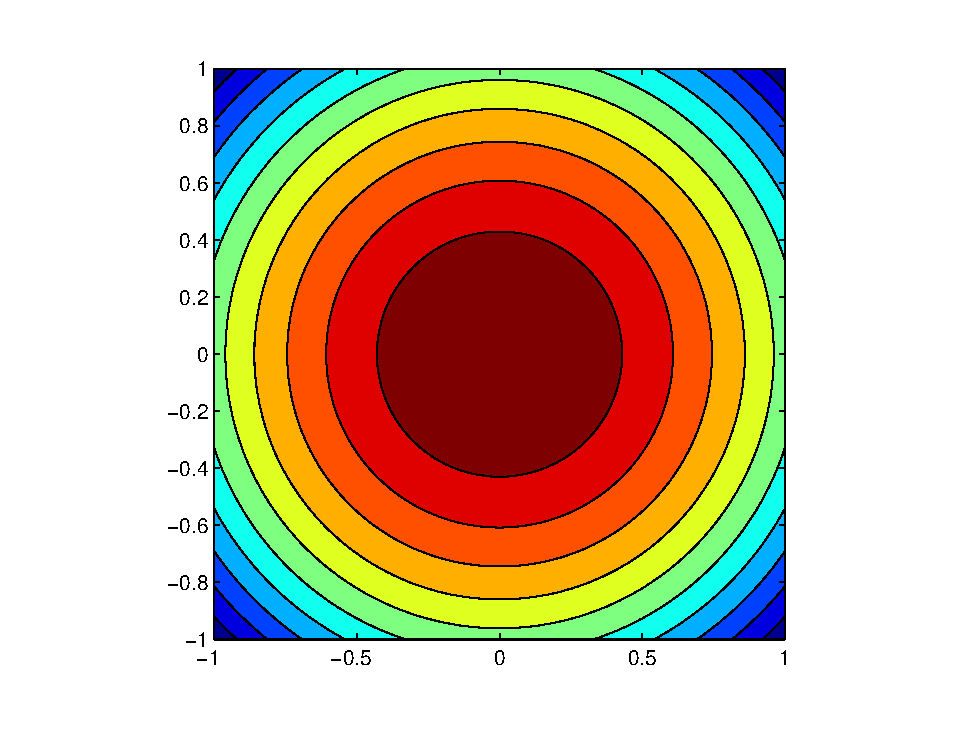
\includegraphics[width = 7cm]{images/courbes.eps}
\caption{$1-k div_i$ for two characteristics and one object according to $r_{j1}$ and $r_{j2}$}
\end{figure}

\subsection{Interpretation}
We can also develop the expression of the energy function $E(r)$ and rewrite it as
$$ E(r) = \sum_{i=1}^N div_i - k \frac{div_i^2}{2} + c$$
If we take $c = \frac{2N}{k}$
Indeed, we then have $$ \sum_{i=1}^N div_i - k \frac{div_i^2}{2} + \frac{2N}{k}= -\frac{1}{2k}(1 - 2kdiv_i + div_i^2)$$
\\
The minimisation of the energy function is actually the minimisation of $  -\frac{1}{2k} w^Tw $.
So the method will actually find the reputation that will maximize the norm 2 of the weight vector. So it will favour a few large weights over more average weights. In other words, we maximize some kind of confidence but we want to be able to know which judges are to be trusted more.


\subsection{Uniqueness of the stationary point}

We can prove that the stationary point corresponding to our problem is unique under some assumptions on $k$.
We need $$k\in \mathcal{K} = \{k\in \mathcal{R}_{\geq 0} | 1 - k \begin{pmatrix} div_1 \\ div_2 \\ \vdots \\ div_n \end{pmatrix} >0 \: \forall r \in \mathcal{H} \}$$
where $\mathcal{H}$ is an hypercube. This ensures that the weights of the ratings are always positive. 

 Since $w$ has elements dependent in $r_{jk}^2$, the energy function is a polynomial of maximum order $4$ in each $r_{jk}$

There is a lemma in \cite{Cristo1} that goes as follows
\begin{lemma}
Let the function $E(r) : \mathbb{R}^n \rightarrow \mathbb{R} : E(r) = z $ be a fourth-order polynomial and let $\mathcal{H}$ be some hypercube in $\mathbb{R}^n$. If 
$$\lim_{||r||\rightarrow \infty} E(r) = - \infty $$
and the steepest descent direction on the boundary of $\mathcal{H}$ points strictly inside $\mathcal{H}$, then $E$ has a unique stationary point in $\mathcal{H}$ which is a minimum.
\label{eq:poly}
\end{lemma}
\todo[inline]{Probleme dans la démo du lemme}
From which follows the following theorem
\begin{theorem}
If $k \in \mathcal{K}$, the system has a unique fixed point $r^{\star}$.\label{thm:uni}
\begin{proof}
The proof is similar to the uni-variable case. If any rating of a judge is the unique rating for an object and characteristic and is on the boundary of $\mathcal{H}$, we can exclude it from the iteration since we know that neither its corresponding reputation nor its participation in the weight of the judge will change over iterations. Hence we suppose that any object and characteristic receives at least two different votes. In that case, since we know that the votes belong to $\mathcal{H}$, we can say that the reputations at any point of the iteration will be in $int(\mathcal{H})$.
We also see that at any point on the boundary the next point will be in $int(\mathcal{H})$. Since the iteration corresponds to a steepest descent step for the energy function, we can say that the gradient on the boundary of $\mathcal{H}$ points inside $\mathcal{H}$. Since when $||r|| \rightarrow \infty$ the weights become infinitely negative, the Energy function satisfies the hypothesis of lemma \ref{eq:poly}. So there is a unique stationary point which is the fixed point of our system.
\end{proof}

\end{theorem}
We note that it is more likely in our multi-variate case to have some unique rating for some characteristic for an object. However, the given rating will determine the final reputation since the change in the weight of the judge won't change the reputation.
\subsection{Convergence}
By an argument similar to what is described in \cite{Cristo1}, we get the convergence result.
We will now prove the convergence of the method towards the unique minimizer of the energy function. In order to do that, we first need to prove a lemma :
\begin{lemma}
Let $c\in \mathbb{R}^{M \times K}$ a second order tensor, $M\in \mathbb{R}^{N\times M \times K}$ and $A\in \{0,1\}^{N\times M \times K}$ be third order tensors so that for $(i,j,k) \in \{1..N \times 1..M \times 1..K \}$ we have $M_{ijk} A_{ijk} = M_{ijk}$. ($M$ is the adjacency matrix of the votes).\\
Then we have 
$$\sum_{j=1}^M \sum_{k=1}^K (M_{ijk}-A_{ijk} c_{jk})^2 = \sum_{j=1}^M \sum_{k=1}^K M_{ijk}^2 - 2\sum_{j=1}^M \sum_{k=1}^K M_{ijk}c_{jk} + \sum_{j=1}^M \sum_{k=1}^K A_{ijk} c_{jk}^2$$
\begin{proof}
We simply use the hypothesis that $M_{ijk}A_{ijk} = M_{ijk}$ :
\begin{eqnarray*}
\sum_{j=1}^M \sum_{k=1}^K (M_{ijk}-A_{ijk} c_{jk})^2 & = & \sum_{j=1}^M \sum_{k=1}^K A_{ijk}(M_ijk-c_jk)^2 \\
& = & \sum_{j=1}^M \sum_{k=1}^K A_{ijk} (M_{ijk}^2 - 2 M_{ijk}c_{jk} + c_{jk}^2)\\
& = & \sum_{j=1}^M \sum_{k=1}^K M_{ijk}^2 - 2\sum_{j=1}^M \sum_{k=1}^K M_{ijk}c_{jk} + \sum_{j=1}^M \sum_{k=1}^K A_{ijk} c_{jk}^2
\end{eqnarray*}
\end{proof}
\label{lemma:tens}
\end{lemma}

Now in order to show that the iteration does converge we will first show that the energy function decreases with the iterations.
\begin{lemma}
For the iteration described in equations \ref{eq:rep} and \ref{eq:w8} and the energy function defined as in equation \ref{eq:energy}, for an iteration $t\in \mathbb{N}$, we have 
$$(w^{t+1})^Tw^{t+1} \geq (w^t)^Tw^t$$
\begin{proof}
We will first express $w^{t+1}$ as a function of $w^t$.
Let $A$ be the adjacency tensor of the votes ($1$ if there is a vote, $0$ if not). Let $M = X - R^t$ with $X$ the tensor of the votes and $R^t_{ijk} = r^t_{jk}$ and let $c = r^{t+1}-r^{t}$. We can see that $A,M$ and $c$ all satisfy the hypothesis of lemma \ref{lemma:tens}.\\
Now let us remember that 
$$w_i^{t+1} = 1 - k \frac{1}{MK} \sum_{j=1}^M \sum_{k=1}^K A_{ijk}(X_{ijk}-r_{jk})^2$$
which can be replaced by
\begin{eqnarray*}
w^{t+1} & = & 1 - \frac{k}{MK} \sum_{j=1}^M \sum_{k=1}^K  (M_{ijk} - A_{ijk}c_{jk})^2\\
& = & 1- \frac{k}{MK}\left[ \sum_{j=1}^M \sum_{k=1}^K (M_{ijk})^2 - 2 \sum_{j=1}^M \sum_{k=1}^K c_{jk}M_{ijk} + \sum_{j=1}^M \sum_{k=1}^K  c_{jk}^2 \right]\\
& = & 1 - \frac{k}{MK}\left[ \sum_{j=1}^M \sum_{k=1}^K (X_{ijk}-r_{jk}^t)^2  - 2 \sum_{j=1}^M \sum_{k=1}^K (r^{t+1}_{jk}-r^t_{jk})(X_{ijk}-r^t_{jk}) \right.\\
& & \left. + \sum_{j=1}^M \sum_{k=1}^K  (r^{t+1}_{jk} - r^t_{jk})^2 \right]\\
& = & w^t + \frac{k}{MK} q
\end{eqnarray*}
with $q = 2 \sum_{j=1}^M \sum_{k=1}^K (r^{t+1}_{jk}-r^t_{jk})(X_{ijk}-r^t_{jk}) - \sum_{j=1}^M \sum_{k=1}^K  (r^{t+1}_{jk} - r^t_{jk})^2 $
\end{proof}
\end{lemma}

As a consequence, we have
\begin{eqnarray*}
(w^{t+1})^Tw^{t+1} & = & (w^t)^Tw^t + \frac{k^2}{M^2K^2} q^Tq + 2 \frac{k}{MK} q^T w^t
\end{eqnarray*}
We need to show that $q^Tw^t \geq 0$.

\begin{eqnarray*}
q^Tw^t & = & 2 \sum_{i=1}^N w^t_i (\sum_{j=1}^M \sum_{k=1}^K (r^{t+1}_{jk}-r^t_{jk})(X_{ijk}-r^t_{jk}) - \sum_{i=1}^N w^t_i \sum_{j=1}^M \sum_{k=1}^K  (r^{t+1}_{jk} - r^t_{jk})^2)\\
& = & \sum_{j=1}^M \sum_{k=1}^K (r^{t+1}_{jk}-r^t_{jk}) \sum_{i=1}^N w^t_i (X_{ijk}-r_{jk}^t)- (\sum_{i=1}^N w^t_i) \sum_{j=1}^M \sum_{k=1}^K  (r^{t+1}_{jk} - r^t_{jk})^2)\\
& = & (\sum_{i=1}^N w^t_i) \sum_{j=1}^M \sum_{k=1}^K  (r^{t+1}_{jk} - r^t_{jk})^2)\\
& \geq & 0
\end{eqnarray*}
We used here the fact that $\sum_{i=1}^N w^t_i (X_{ijk}-r_{jk}^t) = (\sum_{i=1}^N w^t_i) \sum_{j=1}^M \sum_{k=1}^K  (r^{t+1}_{jk} - r^t_{jk})^2)$ by definition of the reputations.
We also have 
$$E(r^{t+1})- E(r^t) \leq \frac{-\delta}{MK} \sum_{j=1}^M \sum_{k=1}^K (r^{t+1}_{jk} - r^t_{jk})^2$$
We know that the sequence of the $r^t$ will not go out of $int(\mathcal{H})$.
Since $E$ is lower bounded on $int(\mathcal{H})$ and that $E$ decreases at each iteration, the sequence will converge. We know also from \ref{thm:uni} that we have converged to the unique minimum of $E$ in $int(\mathcal{H})$



\todo[inline]{introduce sparsity}


\subsection{Sparsity pattern}

This section extends some previous results to the case where the rating matrix has some sparsity pattern, that is when en object is not evaluated by all raters and/or not on all characteristics. Indeed, the structure of real data is sparse. If we take the example of teachers who rate the students on various courses that represent characteristics, it is clear that teacher will rate only their own course and not those of other teachers. We hardly find a set of raters, objects and characteristics with a vote for all possible values.\\

An absence of vote for object $i$ from rater $j$ on characteristic $k$ will imply that the entry $(i, j, k)$ of the tensor $X$ is equal to zero (The reverse is not true). That is, by using the adjacency tensor $A \in \mathbb{R}^{N \times M \times K}$, if $A_{ijk} = 0$, then $X_{ijk}$ = 0. These entries must not be considered as votes but instead as missing values. Therefore the previous equations presented in matrix form require some modifications that will include the adjacency tensor $A$.


\subsubsection{Iterative filtering systems}
 The column vector $d_k^{ij}$ defined in section \ref{section:sub:iteration} becomes
 
\[
    d^{ij}_k = X_{ijk} - A_{ijk}   \circ r_{jk}
\]

\todo[inline]{Je pense qu'on doit diviser ici mais je suis pas trop sûr de par quoi on doit diviser ? Avant on divisait par le nombre d'objects évalués par le juge i. Ici vu que i et j sont fixés, ont devrait diviser par le nombre de charactéristiques évaluées ?}

This latest vector can be seen as the distance of the ratings of the judge $i$ for object $j$ from the reputation of the object $j$ on evaluated characteristics.

\subsubsection{Quadratic iterative filtering systems}

The reputation matrix $F(w, X)$ is now given by

\[
    F_{jk}(w, X) = \frac{\sum_i x_{ijk}w_i}{\sum_i A_{ijk}w_i}
\]

It is simply the sum of the characteristics ratings weighted by the weights of all the judges on this characteristics. Lut us remark that the denomintaor must be strictly positive. This means that every characteristics is evaluated by at least one rater with nonzero weight !

\todo[inline]{On ne divise bien que par le poids des juges qui ont cotés cette charactéristique là ? Dans notre exemple avec les points c'est un peu bizarre vu qu'il n'y a qu'un seul juge pour chaque charactéristique. Dans l'exemple des hotels il est évident que plusieurs personnes peuvent coter une charactéristique.}





\section{Extensions and particular cases}
\subsection{Total score and weighting of characteristics}
At some point it is often expected from a reputation system that it provides a final score for an object. This score can be weighted according to some new parameters $p_k$, each relative to a characteristic.
The first option to account for this is to simply compute the reputations for each characteristic and then perform a weighted sum.
$$ s_j = \sum_{k=1}^K p_k r_{jk} $$
A second option would be to include directly the weighting of the votes inside the calculation of the reputations. We can do this by first multiplying the votes $X_{ijk}$ by the weighting $p_k$. 
$$X'_{ijk} = p_k X_{ijk}$$
This way we will make the ratings in the characteristics with higher ratings more important. It means that an incoherent rating in one of those important ratings will be very penalizing for a judge. This variant can be chosen if we do want to implement that.
The final rating will be calculated as the sum of the resulting $r'_{jk}$s
$$ s_j = \sum_{k=1}^K r'_{jk}$$

\subsection{Interdependence of some characteristics}
Suppose that one judge is the only one to give some object a rating. If this is the case for all the objects, all the weights will be equal to $1$.\\
A way to avoid this is by introducing some dependence between the characteristics of the objects.\\
We keep the usual computation of the reputations as the weighted sum of the ratings as in equation \ref{eq:rep}. The weights would need to be modified. We keep equation \ref{eq:w8} but we modify the definition of $div_i$.
$$div_i = \sum_{j=1}^N \sum_{k=1}^K A_{ijk} \sum_{k2=1}^K l_{k,k2} (X_{ijk}-r_{jk2})^2$$
Where $l_{k,k2}$ represents a dependence between two characteristics. This way, if there is only one rating in one characteristic, the weight of the judge who gave this rating will be influenced by the other reputations.

\subsection{Several judges agree on one rating}
If several judges give a common rating to one object, we can assume that the rating given is the result of the mean of the ratings that each judge would have given separately. At first we simply put the value of the rating in each of the rating of the judges. We can see that this rating will given more weight since it is given by several judges. So we can assume that the weights of the judges will increase compared to the case where a judge is alone to give a rating. However, should we not decrease the influence of this rating?

Ideas :

- Make the combination of the judges a new judge

- Rise the variance used for this rating.
\section{Cheating}

Question : What are the cases where the cheater doesn't know which value to give in order to maximize a final rating? We suppose that when a judge already has many votes, his weight will diminish very slowly when he recedes from the reputation of the object. We expect that there will be cases where the function of a final rating according to a certain rating will be monotonous. In those cases, the optimal behaviour for the cheater is trivial.

\subsection{Intuitive cheating}
The cheater who would want to increase the reputation of one object in one characteristic would be tempted to simply rise his rating for this object and characteristic. It is indeed a good first step as we will show.\\

Let's take as usual a tensor of ratings $X$ and a matrix of reputations $r^{\star}$ that corresponds to the minimum of the energy function. Now we assume that judge $t$ wants to rise the reputation for characteristic $k$ of object $j$. In order to do so, we suppose that he only changes the rating $X_{tjk}$. We will show that increasing $X_{tjk}$ systematically increases the reputation $r_{jk}$.


Let's say that the modified tensor $X'$ is equal in all ratings to $X$, except in $(t,j,k)$. The resulting modified reputation matrix is $r'$. The new energy function relative to the modified ratings is $E'(r')$.
\begin{lemma}
The vector of reputation for the initial ratings $r^{\star}$ is actually the minimum of the new energy function subject to the constraint that $r'_{jk}=r^{\star}_{jk}$.

\begin{align*} 
 & E'(r^{\star}) = \min_{r'} E'(r')\\
s.t.  & \:\: r'_{jk} = r_j
\end{align*}

\begin{proof}
The Lagrangian of the problem can be written as
$$\mathcal{L}(r') = E'(r') + \lambda (r'_{jk} - r_{jk}^{\star})$$

$$\frac{\partial E'}{r'_{jk}} = \sum_{i=1}^N w_i (-2 (X'{ijk}-r'_{jk})$$
We know that $\nabla_{r'}E'(r') = \begin{pmatrix} 0 & \hdots & -2 (X'_{tjk}-X_{tjk})w^t & \hdots & 0\end{pmatrix}^T$
As discussed before, there cannot be local minimas or maximas or saddle points \todo[inline]{Check the proof of the article}.
We can see that the Karush-Kuhn-Tucker conditions are satisfied for $r' = r^{\star}$ and $\lambda = 2 (X'_{tjk}-X_{tjk})w^t$. So $r^{\star}$ is the minimum for $r'_{jk} = r^{\star}_{jk}$
\end{proof}
\end{lemma}


\begin{proposition}
An increase in $X_{tjk}$ automatically leads to an increase in $r_{jk}$
\begin{proof}
When we compute the new reputation, we can start the iteration from the former $r^{\star}$. At this point, we know that $r'_{jk}$ will increase since $\frac{\partial E'}{r'_{jk}} $ is negative. So we have $(r'_{jk})^2 > r^{\star}_{jk}$
So now let's suppose that $(r'_{jk})^{\star}< r^{\star}_{jk} $. Since $E'$ diminishes at every iteration it would imply that there is a saddle point in $H$
\end{proof}

\end{proposition}
Idea : 

-maximize the ratio of 2 reputations

-Quid de la moyenne?
\bibliographystyle{plain}
\bibliography{rapport/bib/biblio}
\nocite{*}


\end{document}